
%=====================================================================
%CAPITULO I
%=======================================================================
\chapter{Cardinalidad} En esta unidad estudiaremos el concepto de
cardinalidad de un conjunto. Con este concepto se pretende darle
un entendimiento a la noci\'on de cantidad de elementos de un
conjunto, en especial cuando este es ``infinito''. Como se ver\'a,
y por extra\~no que parezca, aunque el conjunto involucrado sea
``infinito'', de todas maneras podremos definir el cardinal de ese
conjunto, con esto implicitamente decimos que no todos los
conjuntos infinitos tendr\'an el mismo cardinal. Empezaremos
recordando algunas cuestiones b\'asicas de teor\'{\i}a de
conjuntos que, a la vez, nos servir\'an como referencia para  las
notaciones.

%--------------------------------------------------------------
%SECCION




\section{Repaso de lo b\'asico sobre conjuntos}
La siguiente introducci\'on est\'a lejos de ser exhaustiva, solo
recordaremos conceptos ya sabidos. Nos dentendremos algo m\'as en
aquellos puntos que puedan ser nuevos.

\begin{definicion}Dados dos conjuntos $A$ y $B$ denotaremos su uni\'on,
intersecci\'on y diferencia por: $A\cup B$, $A\cap B$ y $A-B$
repectivamente. Estos nuevos conjuntos se definen por:
\[A\cup B=\{x:x\in A\vee x\in B\},\]

\[A\cap B=\{x:x\in A\wedge x\in B\}\]
y

\[A-B=\{x:x\in A \wedge x\notin B\},\]
respectivamente.
\end{definicion}
 Por lo general, tendremos que los
conjuntos con los que trabajaremos estar\'an contenidos en un
conjunto que llamaremos el universo $\mathcal{U}$. Aceptado la
existencia de este universo, frecuentemente usaremos la siguiente
notaci\'on para el complemento
\[A^c=\mathcal{U}-A.\]
Adem\'as consideraremos la operaci\'on de diferencia sim\'etrica,
defini\'endose esto por:
\[A\bigtriangleup B=(A-B)\cup(B-A).\]

\begin{definicion}Dados dos elementos arbitrarios $a$ y $b$ se
define el par ordenado $(a,b)$, por la siguiente igualdad
\[(a,b)=\{a,\{a,b\}\}.\]
\end{definicion}

La propiedad m\'as relevante de pares ordenados es que si
$(a,b)=(c,d)$ entonces $a=c$ y $b=d$. Ahora consideramos el
conjunto formado por todos los pares ordenados de elementos
pertenecientes a conjuntos dados.

\begin{definicion} Sean $A$ y $B$ conjuntos. El producto cartesiano de $A$ con
$B$, denotado por $A\times B$, es el siguiente conjunto:
\[A\times B=\{(a,b):a\in A\wedge b\in B\}.\]
\end{definicion}
La siguiente definici\'on es bien conocida.

\begin{definicion} Una funci\'on $f$ de $A$ en $B$ (abreviaremos esta frase
porel siguiente s\'{\i}mbolo: $f:A\longrightarrow B$), es un
subconjunto del producto cartesiano $A\times B$ con la propiedad
que: para todo $a\in A$ existe un \'unico $b\in B$ tal que
$(a,b)\in f$. \end{definicion}

Suponemos que ya todos conocemos estos conceptos, asi como los
conceptos relacionados de: imagen, la notaci\'on $f(a)$, funci\'on
inyectiva, suryectiva y biyectiva. Admitimos todo esto por sabido.
Ahora introducimos una nueva notaci\'on.

\begin{definicion}
Por $B^A$ denotamos al conjunto de todas las funciones
$f:A\longrightarrow B$.
\end{definicion}

Mas adelante daremos algunas explicaciones del porque de esta
notaci\'on.

Seguidamente damos las definiciones, que pueden no haberse usado
antes, de los conjuntos imagen y preimagen, de un conjunto dado,
por una funci\'on, tambi\'en, dada.

\begin{definicion} Dada una funci\'on $f:A\longrightarrow B$ y subconjuntos
$C\subset A$ y $D\subset B$ definimos:
\[f(C)=\{f(a):a\in C\}\]
y
\[f^{-1}(D)=\{a\in A:f(a)\in C\}.\]
\end{definicion}

Las figuras \vref{figura1} y \vref{figura2} aclaran el significado
de estos conjuntos.


\begin{figure}[h]

\begin{center}

\psfrag{A}{$A$}

 \psfrag{B}{$B$}

 \psfrag{C}{$C$}
 \psfrag{f(C)}{$f(C)$}
 \psfrag{f}{$f$}


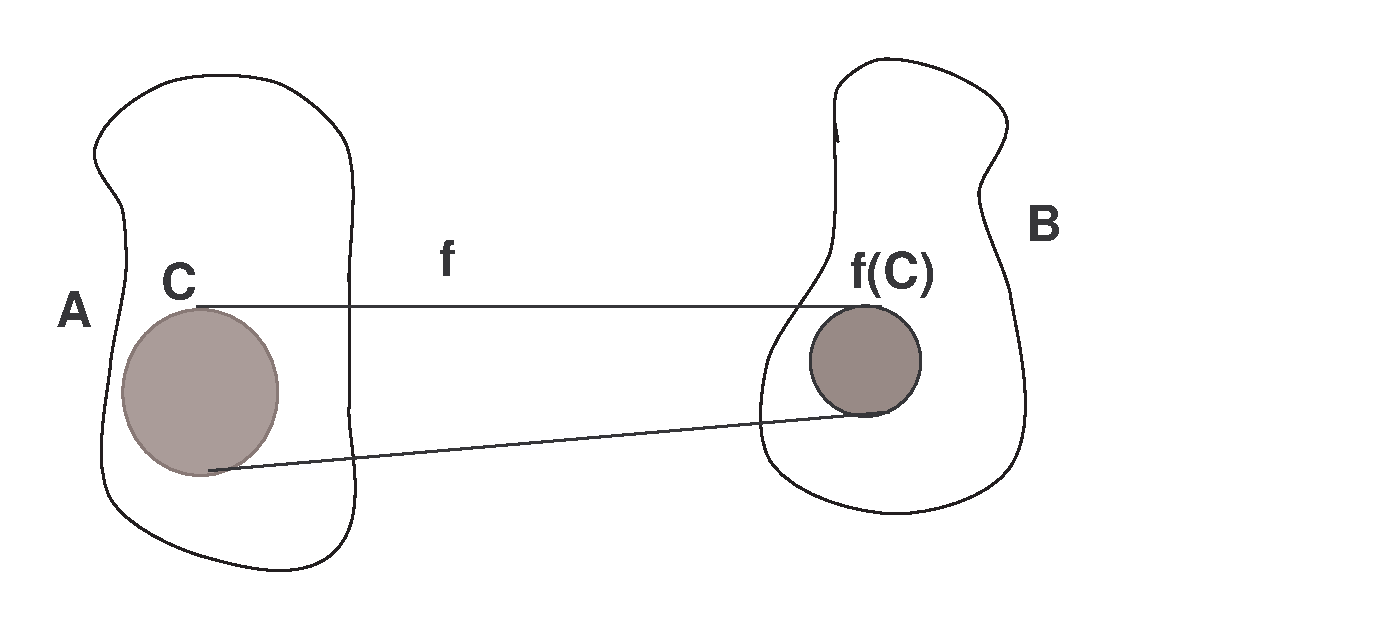
\includegraphics[height=5cm, width=10cm]{funcima.eps}


 \caption{Conjunto $f(C)$}\label{figura1}

\psfrag{A}{$A$}

 \psfrag{B}{$B$}

 \psfrag{D}{$D$}
 \psfrag{f-1(D)}{$f^{-1}(D)$}
 \psfrag{f}{$f$}


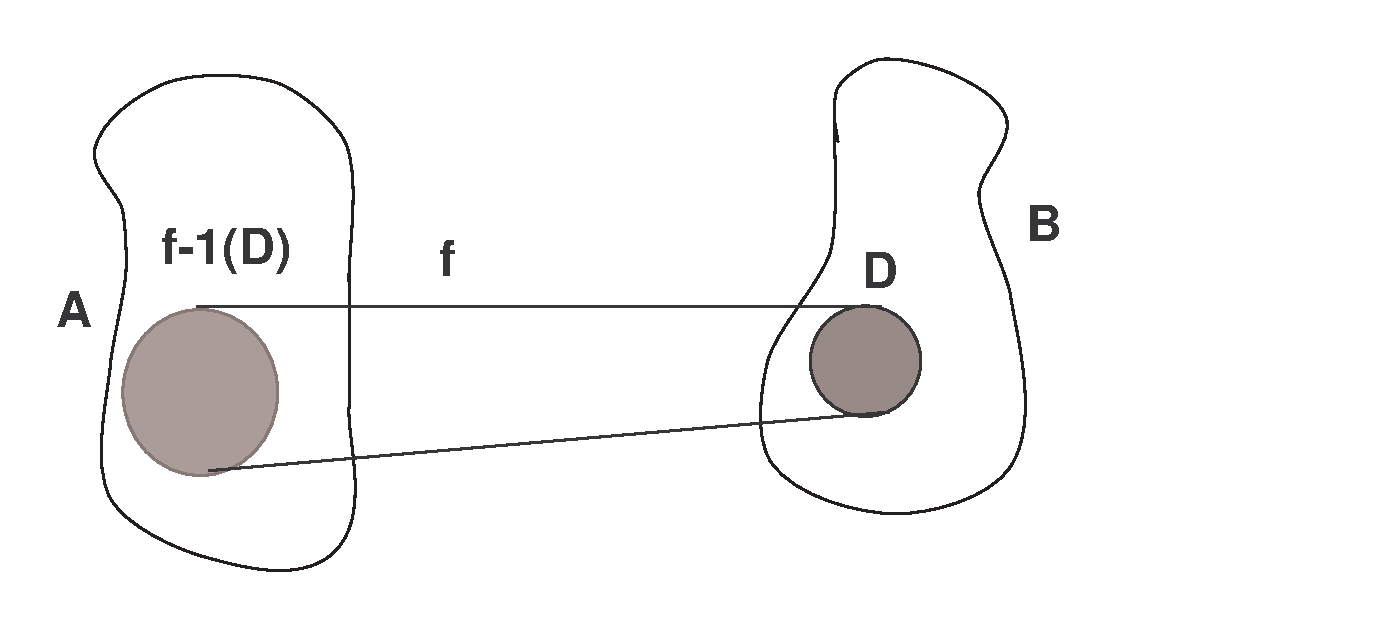
\includegraphics[height=5cm, width=10cm]{fpreima.eps}


 \caption{Conjunto $f^{-1}(D)$}\label{figura2}


\end{center}

\end{figure}





Muy a menudo utilizaremos las propiedades que a continuaci\'on se
enuncian. Las demostraciones, de las mismas, quedaran a cargo del
alumno; ver Ejercicio \vref{3}.

\begin{proposicion}\label{propfunc} Sea $f:A\longrightarrow B$ una funci\'on.
Entonces
\begin{itemize}
\item[1.] $f(C_1\cup C_2)=f(C_1)\cup fe(C_2).$
\item[2.]$f^{-1}(D_1\cup D_2)= f^{-1}(D_1)\cup f^{-1}(D_2).$
\item[3.] $f(C_1\cap C_2)\subset f(C_1)\cap f(C_2).$
\item[4.]$f^{-1}(D_1\cap D_2)= f^{-1}(D_1)\cap f^{-1}(D_2).$
\end{itemize}
\end{proposicion}


Tambi\'en vamos a considerar el conjunto de partes de un conjunto
dado, esto es el conjunto de todos sus subconjuntos.
Expl\'{\i}citamente:
\[\mathcal{P}(A)=\{C:C\subset A\}.\]
Se pueden efectuar uniones e intersecciones de una cantidad
arbitraria de conjuntos. Para poder enunciarlas debemos definir
antes lo que entendemos por una \emph{familia subindicada de
conjuntos} (o brevemente \emph{familia de conjuntos}).

\begin{definicion} Supongamos dado un conjunto $I$, al que nos referiremos como
conjunto de \'{\i}ndices, y una funci\'on $F:I\longrightarrow
\mathcal{P}(A)$. As\'{\i} tenemos que, para cada $i\in I$, existe
un \'unico subconjunto de $A$, que llamaremos\footnote{Observar
que esto es posible puesto que tenemos una dependencia funcional
de los subconjuntos de $A$ con los elementos de $I$} $A_i$ tal que
$f(i)=A_i$. Diremos entonces que $\{A_i\}_{i\in I}$ es una familia
subindicada de conjuntos por el conjunto de \'{\i}ndices $I$.
\end{definicion}

Ahora podemos definir la uni\'on y la intersecci\'on de una
familia de esta \'{\i}ndole de la siguiente manera
\begin{definicion} Definimos la uni\'on e intersecci\'on de una
familia $\{A_i\}_{i\in I}$ por:
\[\bigcup_{i\in I}A_i=\{a:\exists i\in I:a\in A_i\}\]
y
\[\bigcap_{i\in I}A_i=\{a:\forall i\in I:a\in A_i\}\]
respectivamente.
\end{definicion}
En el Ejercicio \vref{propuniarb} podemos encontrar una seria de
propiedades de uniones e intersecciones de familias de conjutos.
Estas propiedades las usaremos con frecuencia.
 Por \'ultimo, en esta revisi\'on de conjuntos, expondremos el
 axioma de elecci\'on. Este es un axioma de la teor\'{\i}a de
 conjuntos. Hay que aclarar que es posible axiomatizar la
 teor\'{\i}a de conjuntos, de esta axiomatizaci\'on el mencionado axioma
 puede formar parte. Decimos ``puede'' por que este
 axioma ha despertado multitud de controversias en torno a su
 inserci\'on o no en el restante conjunto de axiomas. No vamos a
 discutir aqu\'{\i} esta controversia ni tampoco la teor\'{\i}a
 axiom\'atica de conjuntos pues esto nos desviar\'{\i}a de nuetros
 objetivos. Solo enunciaremos el axioma de elecci\'on, que
 usaremos frecuentemente.

\begin{axioma} Sea $\{A_i\}_{i\in I}$ una familia de conjuntos no
vacios. Entonces existe una funci\'on
\[f:I\longrightarrow\bigcup_{i\in I}A_i.\]
con la propiedad  que: $\forall i\in I$
\[f(i)\in A_i.\]
\end{axioma}



%--------------------------------------------------------------
%SECCION


\section{Definici\'on de conjuntos coordinables}
En esta secci\'on definimos el concepto clave de esta unidad, a
saber el concepto de que dos conjuntos sean coordinables. Damos
una breve discuci\'on para motivar nuestra definici\'on.

 Cuando
algui\'en cuenta alg\'un conjunto de cosas, establece una
correspondencia entre los objetos que cuenta y un subconjunto de
n\'umeros naturales... veamos como. En el proceso de conteo,
alg\'un objeto fue el primero en contarse, y se habr\'a dicho:
``uno'' para ese objeto. El proceso continua asignando,
sucesivamente, el n\'umero dos, tres, etc, a los restantes objetos
a contar, hasta que no queden m\'as por contarse. As\'{\i}, si en
este proceso llegamos hasta el 20, por ejemplo, decimos que hay 20
objetos. Aunque no haya que percatarse de eso a los fines
pr\'acticos, lo que tambi\'en hicimos fue: Establecer una
correspondencia o funci\'on entre los objetos y el conjunto
$\{1,\dots,20\}$. M\'as a\'un, esta correspondencia fue biyectiva
pues: A cada n\'umero le correspondi\'o solo uno de los objetos
(es decir: La funci\'on es inyectiva) y a cada objeto le
correspondi\'o alg\'un n\'umero (es decir: La funci\'on es
suryectiva). En otras palabras contar un conjunto significa:
determinar el \emph{intervalo inicial del conjunto} de los
n\'umeros naturales\footnote{Por esto se entiende un conjunto de
la forma: $\{j\in\mathbb{N}:1\leq j\leq n\}$, para cierto
$n\in\mathbb{N}$. De ahora en m\'as, llamaremos a este conjunto:
$\mathbb{N}_n$} para el cual exista una correspondencia biyectiva
con el conjunto que queremos contar. Conocer esto obviamente es
in\'util a los efectos de contar cosas de la ``vida cotidiana'';
no obstante, es una observaci\'on fundamental a los efectos de
extender lo que llamamos ``contar'' a conjuntos infinitos. Lo que
antecede sugiere la siguiente definici\'on.

\begin{definicion}\label{defcoordinables} Dados dos conjuntos: $A$ y $B$,
se dir\'a que ellos son coordinables, escribiremos $A\thicksim B$,
si existe una funci\'on biyectiva $f:A\longrightarrow B$.
\end{definicion}

Esta es nuestra definici\'on de que dos conjuntos, ``finitos'' o
no, tengan ``la misma cantidad de elementos''. Como veremos, no
todos los  conjuntos ``infititos'' son coordinables entre si.

Es bueno notar que no es dif\'{\i}cil demostrar que $\thicksim$ es
una relaci\'on de equivalencia (ver Ejercicio \vref{1}).

 Ahora
veamos algunos ejemplos.

\begin{ejemplo}Consideremos la funci\'on
$f:\nn\longrightarrow\{x\in\nn:x\,\,\text{es par}\}$, definida por
$f(x)=2x$. Facilmente se ve que $f$ es una biyecci\'on entre los
conjuntos indicados. De ah\'{\i} que:
$\nn\thicksim\{x\in\nn:x\,\,\text{es par}\}$.
\end{ejemplo}

En este ejemplo observamos que, desde nuestro punto de vista, el
conjunto de los naturales tiene ``la misma cantidad de elementos''
que el conjunto de los naturales pares. Es decir, en este caso, el
todo no es mayor que una de sus partes.

\begin{ejemplo}\label{rcoord(0,1)} Veamos que $\rr\thicksim (0,1)$. En este caso se
puede considerar la funci\'on

\[f(x):= \tan\biggl(\frac{2\pi x-\pi}{2}\biggr).\]
Dejamos como ejercicio corroborar que la funci\'on dada establece
una biyecci\'on entre los conjuntos involucrados.
\end{ejemplo}

Los dos ejemplos anteriores muestran una caracter\'{\i}stica
importante de los conjuntos ``infinitos''; un subconjunto de ellos
puede ser coordinable con el conjunto total. Mientras que, los
conjuntos ``finitos'' parecen carecer de esta caracter\'{\i}stica.
Ver Ejercicio \vref{infcoordconsub}




%--------------------------------------------------------------
%SECCION

\section{Conjuntos numerables}
Hasta el momento empleamos comillas para encerrar los t\'erminos:
finito e infinito. Esto se debe a que estamos en condiciones, a
partir de la noci\'on  de coordinalidad, de definir de forma
precisa el significado de estos t\'erminos.

\begin{definicion} Diremos que un conjunto $A$ es:
\begin{itemize}
\item[1.] \textbf{finito} si existe un $n\in\nn$ tal que
$A\thicksim\nn_n$.
\item[2.] \textbf{infinito }si no es finito.
\item[3.] \textbf{numerable} si $A\thicksim\nn$.
\item[4.] \textbf{a lo sumo numerable} si es finito o numerable.
\end{itemize}
\end{definicion}

En virtud de que $\thicksim$ es una realci\'on de equivalencia, y
especialmente por el car\'acter transitivo de esta, si $A\thicksim
B$ y $B$ tiene alguna de las cuatro propiedades de la definici\'on
anterior entonces $A$ tendr\'a esa misma propiedad.

Recordemos que, por definici\'on, una sucesi\'on $\{a_i\}$ de
elementos de un conjunto $A$ es una funci\'on
$f:\nn\longrightarrow A$, donde $a_i=f(i)$. Vemos as\'{\i} que el
concepto de numerabilidad est\'a relacionado con el de sucesi\'on.
En efecto, si el conjunto $A$ es numerable entonces sus elementos
se pueden disponer en una sucesi\'on, donde ning\'un t\'ermino se
repita.

Es oportuno que observemos que un conjunto no puede ser numerable
y finito a la vez; dicho de otra forma, los conjuntos numerables
son infinitos. Esto, como hemos definido los conceptos numerable y
finito de  manera precisa, tiene que ser demostrado.

\begin{teorema}\label{nesinfinito} Un conjunto numerable es
infinito.
\end{teorema}
\begin{demo} Supongamos que, por lo contrario, existe un conjunto
$A$ numerable y, a la vez, finito. As\'{\i} tendr\'{\i}amos que:
$A\thicksim\nn$ y $A\thicksim\nn_n$, para alg\'un $n\in\nn$. Como
$\thicksim$ es una relaci\'on de equivalencia , deducimos que
$\nn\thicksim\nn_n$. Sea, pues, $f$ una biyecci\'on:
$f:\nn_n\longrightarrow\nn$. Ahora consideremos el
natural\footnote{El s\'{\i}mbolo $:=$ se lee \emph{igual por
definici\'on}. Esto es, el miembro de la izquierda es definido por
el de la derecha}: $k:=f(1)+\dots+f(n)+1$. Como $f$ es una
biyecci\'on, existe alg\'un $m$, con $1\leq m\leq n$ tal que
$f(m)=k$. Es decir
\[f(m)=f(1)+\dots+f(n)+1.\]
Seguramente, en el miembro derecho, uno de los t\'erminos es
$f(m)$. Este se puede cancelar con el miembro de la izquierda,
quedando
\[0=f(1)+\dots+f(m-1)+f(m+1)+\dots+f(n)+1.\]
Esta igualdad es absurda pues el miembro de la derecha es mayor
que $1$.
\end{demo}

Vamos a ver algunos otros conjuntos que tambi\'en son numerables.
Empezamos por el siguiente.

\begin{proposicion}\label{subconjunto} Un subconjunto de un conjunto a lo sumo numerable es a
lo sumo numerable.
\end{proposicion}
\begin{demo} Sea $A\subset B$, con $B$ a lo sumo numerable. Se puede suponer
que $B\subset \nn$. ?`Por qu\'e? Y, tambi\'en podemos suponer que
$A$ es infinito, puesto que si fuera finito no habr\'{\i}a nada
que probar. Definimos una funci\'on $f:\nn\longrightarrow A$ por
induccion. Puesto que los n\'umeros naturales son bien ordenados,
tenemos que $A$ tiene un primer elemento, digamos, $a_1$.
Definamos
\[f(1)=a_1.\]
Ahora definimos $f(j)$ por:
\begin{equation}\label{frecursiva}
f(j)=\text{el primer elemento del conjunto: }A-\{f(i):1\leq i\leq
j-1\}. \end{equation} Esta definici\'on es posible pues
$A-\{f(i):1\leq i\leq j-1\}\neq\emptyset$, de lo contrario $A$
ser\'{\i}a finito. Queda as\'{\i} definida la funci\'on $f$. Resta
ver que es biyectiva.

Veamos, en primer lugar, que es inyectiva. Sea $i>j$. En virtud de
~\eqref{frecursiva}, tenemos que $f(i)\notin\{f(k):1\leq k\leq
i-1\}$ de lo cual, y como $j<i$, deducimos que $f(i)\neq f(j)$.

Ahora veamos la suryectividad. Supongamos que existe un elemento
$n\in A$ tal que $n\notin f(\nn)$. Recordemos la Definici\'on
\eqref{frecursiva}. Ella nos dice, en virtud de que $n\notin
f(\nn)$, que $f(i)<n$, para todo $i$. Esto es debido a que $f(i)$
es el m\'{\i}nimo del conjunto $ A-\{f(k):1\leq k\leq i-1\}$ y a
que $n$ pertenece a ese conjunto. Tenemos, entonces, que
$f(\nn)\subset\nn_n$. Como consecuencia del Ejercicio \vref{1.5}
conclu\'{\i}mos que $f(\nn)$ es finito. Pero como $f$ es inyectiva
$\nn\thicksim f(\nn)$. Lo que es una contradicci\'on pues $\nn$ es
infinito.
\end{demo}

\begin{proposicion}\label{zesnum}
El conjuntos $\mathbb{Z}$, de los enteros,  es numerable.
\end{proposicion}
\begin{demo} Constru\'{\i}mos una funci\'on que establece
una biyecci\'on entre: Los enteros positivos y los naturales pares
y entre los enteros negativos y los naturales impares. La
funci\'on es la siguiente:

\[f(x)=\left\{
\begin{array}{ll}
    2x+2, & \hbox{si $x\geq 0$;} \\
    -2x-1, & \hbox{si $x<0$.} \\
\end{array}
\right.\] Dejamos como ejercicio demostrar que, efectivamente, la
funci\'on $f$ es una biyecci\'on entre $\nn$ y $\mathbb{Z}$.
\end{demo}

\begin{proposicion}\label{NxNesnum} El conjunto $\nn\times\nn$ es numerable.
\end{proposicion}
\begin{demo} La demostraci\'on de este enunciado ya no es tan
sencilla. La idea se la debemos a G. Cantor. Daremos una idea de
la construcci\'on de la biyecci\'on entre $\nn\times\nn$
 y $\nn$. En rigor de verdad, a los efectos l\'ogicos de la demostraci\'on, todo lo que sigue
 se podr\'{\i}a obviar; pudi\'endose dar la f\'ormula
 ~\eqref{forfinal} sin dar ninguna justificaci\'on de como se nos
 ocurri\'o. Elegimos el camino contrario, explicar
 como obtener la f\'ormula.


 Dispongamos del conjunto $\nn\times\nn$ en un arreglo del tipo
de una ``matr\'{\i}z infinita'', como sigue:
\[\begin{diagram}
(1,1)   & \rTo        & (1,2)  &                      & (1,3)  &                      & (1,4) &\dots\\
        & \ldTo(2,2)  &        &\ldTo(2,2)\ruTo(4,2)  &        & \ldTo(2,2)\ruTo(6,4) &        &     \\
(2,1)   &             & (2,2)  &                      & (2,3)  &                      &        &      \\
        &\ldTo(2,2)   &        & \ldTo(2,2)           &        & \ddots               &        &      \\
(3,1)   &             &(3,2)   &                      &        &                      &        &      \\
        & \ldTo(2,2)  &        &   \ddots             &        &                      &        &      \\
 (4,1)  &             &        &                      &        &                      &        &      \\
 \vdots &             &        &                      &        &                      &        &      \\
\end{diagram}\]
Notar que, adem\'as de colocar los pares ordenados, hemos colocado
algunas flechas. Estas flechas indican un ``camino''; este es el
camino que seguiremos  para enumerar los pares ordenados.
As\'{\i}, construiremos una funci\'on $f$ que har\'a las
siguientes asignaciones:

\begin{eqnarray}
    f:\nn\times\nn&\longrightarrow\nn\nonumber \\
    (1,1)&\longmapsto 1\nonumber \\
    (1,2)&\longmapsto 2\nonumber \\
     (2,1)&\longmapsto 3\nonumber\\
        &\hspace{-29pt}\vdots\nonumber \\
        \nonumber
\end{eqnarray}
Observar que, en nuestro ``camino'', vamos siguiendo diagonales de
la matriz, de izquierda a derecha y de arriba hacia abajo. Cuando,
siguiendo el camino, llegamos al margen izquierdo de la matriz
``saltamos'' al borde superior, para luego ``descender'' por la
siguiente diagonal. Estas diagonales tienen $1, 2, 3, \dots$
elementos. Agrupemos los n\'umeros naturales de esa forma, es
decir un primer grupo de uno, un segundo de dos y as\'{\i}
indefinidamente:

\[\underbrace{1}_{1} \underbrace{2\quad 3}_{2}\quad\underbrace{4\quad 5\quad
6}_{3}\quad \underbrace{7\quad 8\quad  9\quad 10}_{4}\dots
\]
Obs\'ervese que

\begin{equation}\label{numfinal}
\frac{j(j +1)}{2}=\text{n\'umero final del agrupamiento
$j$-\'esimo}.
\end{equation}
Por ejemplo: el grupo cuarto tiene por su \'ultimo elemento el 10,
que es igual a 4.5/2. Tambien tenemos que todos los pares
ordenados sobre la misma diagonal, tienen la caracter\'{\i}stica
de que sus componentes suman lo mismo. Numeremos las diagonales,
de izquierda a derecha, empezando por 1. As\'{\i} tenemos que la
diagonal 1 posee el elemento (1,1), la diagonal dos tiene los
elementos $(1,2)$ y $(2,1)$, etc. Por lo observado, tenemos la
siguiente f\'ormula, para cualquier par $(j,k)$

\begin{equation}\label{numdiag}
j+k-1=\text{el n\'umero de la diagonal a la que pertenece } (j,k).
\end{equation}
 El objetivo es poner en correspondencia la diagonal
$j$-\'esima con el grupo $j$-\'esimo de naturales. Notar que, en
virtud de ~\eqref{numfinal}, tenemos que
\begin{equation}\label{numdiag2}
\begin{split}\frac{(j+k-1)(j+k)}{2}=&\text{es el \'ultimo n\'umero}\\
 & \text{del agrupamiento $j+k-1$-\'esimo}.\\
\end{split}
\end{equation}
As\'{\i}, si al primer miembro de ~\eqref{numdiag2} le restamos
$(j-1)$, obtenemos el n\'umero que ocupa el lugar $j$ (contando de
atras para adelante) del agrupamiento $j+k-1$ de naturales. Con
esto probamos que la funci\'on que queriamos construir es:


\begin{equation}\label{forfinal}
f(j,k):=\frac{(j+k-1)(j+k)}{2}-j+1.
\end{equation}
Dejamos como ejercicio  demostrar que ~\eqref{forfinal} es
biyectiva (ver Ejercicio \vref{2}).
\end{demo}

Como consecuencia del Ejercicio \vref{1.2} y de la Proposici\'on
anterior, podemos afirmar que si $A$ y $B$ son numerables,
entonces $A\times B$ es numerable.



La siguiente propiedad tambi\'en es \'util para determinar si un
conjunto es numerable.

\begin{proposicion}\label{numinysur}Sean $A$ y $B$ conjuntos, con $B$ a lo sumo
numerable.
\begin{itemize}
\item[1.] Supongamos que existe una funci\'on inyectiva $f:A\longrightarrow
B$. Entonces $A$ es a lo sumo numerable.
\item[2.] Supongamos que existe una aplicaci\'on suryectiva
$f:B\longrightarrow A$. Entonces $A$ es a lo sumo numerable.
\end{itemize}
\end{proposicion}
\begin{demo} Veamos primero 1. La funci\'on $f$ es  una biyecci\'on entre $A$ y su
imagen $f(A)$. Como $B$ es a lo sumo numerable,  y como
consecuencia de la Proposici\'on \vref{subconjunto}, tenemos que
$f(A)$ es a lo sumo numerable. Ahora, como $A\thicksim f(A)$
tenemos que $A$ es a lo sumo numerable.

Ahora probemos 2. Como $f$ es suryectiva, tenemos que $\forall
a\in A$: $f^{-1}(\{a\})\neq\emptyset$. Ahora, por el axioma de
elecci\'on sabemos que existe al menos una funci\'on
$g:A\longrightarrow B$ tal que $\forall a\in A:g(a)\in
f^{-1}(\{a\})$. Si pudi\'eramos probar que la funci\'on $g$ fuera
inyectiva, entonces obtendr\'{\i}amos la tesis a partir del inciso
1, que ya fue demostrado. Veamos, pues, que $g$ es inyectiva.
Supongamos que $a_1,a_2\in A$ y que $a_1\neq a_2$. Afirmamos que
$f^{-1}(\{a_1\})\cap f^{-1}(\{a_2\})=\emptyset$. En efecto, si
$b\in f^{-1}(\{a_1\})\cap f^{-1}(\{a_2\})$ entonces por un lado
 $f(b)=a_1$ y por otro $f(b)=a_2$, lo que es una contradicci\'on pues $a_1\neq a_2$.
\end{demo}

Es interesante hacer notar que, utilizando el teorema anterior,
podemos dar otra demostraci\'on, m\'as concisa, de la
Proposici\'on \vref{NxNesnum}.

En esta demostraci\'on hacemos uso del Teorema Fundamental de la
Aritm\'etica. Recordemos lo que este teorema nos dice:


\begin{itshape}\noindent Todo entero positivo $n$ se representa, de
manera \'unica, de la forma $n=p_1^{\alpha_1}p_2^{\alpha_2}\dots
p_j^{\alpha_j}$, donde $p_1$, $p_2$,...,$p_j$ son n\'umeros primos
y $\alpha_1$, $\alpha_2$,...,$\alpha_j$ son enteros positivos.
\end{itshape}

Definimos la siguiente funci\'on

\[\begin{split}
f:\nn\times\nn&\longrightarrow\nn\\
 (n,m)&\longrightarrow 2^n3^m\\
 \end{split}.
 \]
Por el Teorema Fundamental de la Aritm\'etica, y mas precisamente
por la unicidad de la representaci\'on, tenemos, como $2$ y $3$
son primos, que si $2^n3^m=2^{n^{\prime}}3^{m^{\prime}}$ entonces
$n=n^{\prime}$ y $m=m^{\prime}$. Por consiguiente la funci\'on $f$
es inyectiva. Ahora, invocando la Proposici\'on \vref{numinysur}
conclu\'{\i}mos que $\nn\times\nn$ es a lo sumo numerable. Lo que
resta es, solo, ver que $\nn\times\nn$ no es finito. Esto se puede
probar observando que $\nn\times\nn$ contiene el subconjunto
$A=\{(1,n):n\in\nn\}$ que es coordinable con $\nn$, ?`Cu\'al es la
biyecci\'on?, y por consiguiente infinito. As\'{\i},
$\nn\times\nn$ no puede ser finito, si lo fuera, $A$ tambi\'en lo
ser\'{\i}a, por ser un subconjunto de \'el. Lo que concluye la
demostraci\'on.

Ahora podemos demostrar  uno de los resultados m\'as interesantes
de esta teor\'{\i}a.

\begin{teorema} El conjunto $\mathbb{Q}$, es decir los n\'umeros
racionales positivos, es numerable.
\end{teorema}
\begin{demo} Sabemos que $\mathbb{Z}$ es numerable
y tambi\'en que $\mathbb{Z}\times\mathbb{Z}$ es numerable. Podemos
definir la siguiente funci\'on:
\[
\begin{split}
f:\mathbb{Z}\times\mathbb{Z}&\longrightarrow\mathbb{Q}\\
(n,m)&\longmapsto \frac{n}{m}
\end{split}
.\] Esta aplicaci\'on es suryectiva. Por consiguiente, usando la
parte 2. de la Proposici\'on \vref{numinysur}, obtenemos que
$\mathbb{Q}$ es a lo sumo numerable. Esto es: $\mathbb{Q}$ es
finito o numerable. Pero como $\mathbb{Q}$ es infinito, pues
$\nn\subset\mathbb{Q}$, tenemos que $\mathbb{Q}$ es numerable.
\end{demo}


Traduciendo nuestra interpretaci\'on de que dos conjuntos
coordinables tienen la misma cantidad de elementos, vemos que hay
tantos racionales como naturales. Esta afirmaci\'on es un tanto
desconcertante, en un comienzo. Sabemos que los racionales son
densos dentro de los reales. Esto quiere decir que dentro de cada
intervalo abierto, por chico que este fuere, siempre hay n\'umeros
racionales dentro. Sin embargo, uno puede poner en correspondencia
$\nn$ y $\mathbb{Q}$. Es decir, podemos asignar un racional al
uno, otro al dos y as\'{\i} sucesivamente. En una cantidad
infinita de pasos, podemos poner en correspondencia cada natural
con un \'unico racional y viceverza. A esta altura, pareciera que
todos los conjuntos resultan ser numerables, pero ya veremos, en
la secci\'on siguiente, que no es as\'{\i}.


\begin{lema}\label{subconjnum} Todo conjunto infinito tiene un
subconjunto numerable.
\end{lema}

\begin{demo} Sea $A$ un conjunto infinito. Usaremos un argumento similar a la demostraci\'on de
la Proposici\'on \vref{subconjunto}. Definimos inductivamente una
funci\'on $f:\nn\longrightarrow A$  de la siguiente manera. Puesto
que $A$ es infinito, en particular, es no vacio, as\'{\i} podemos
encontrar un elemento $a_1\in A$. Ponemos entonces
\[f(1)=a_1.\]
Ahora, supongamos que tenemos definida la funci\'on $f$, de tal
manera que sea inyectiva, para $j=1,\dots n$. Llamemos $f(j)=a_j$,
para $j=1,\dots , n$. Como $A$ es infinito no puede ocurrir que
$A-\{f(1),\dots,f(n)\}=\emptyset$, de lo contrario $f$ adem\'as de
ser inyectiva, de $\nn_n$ en $A$, ser\'{\i}a suryectiva; y de este
modo $A\thicksim\nn_n$ lo que implica que $A$ es finito,
contrariando nuestra hip\'otesis. Por consiguiente, podemos
encontrar $a_{n+1}\in A-\{f(1),\dots,f(n)\}$. Definimos
$f(n+1)=a_{n+1}$.

Ahora veamos que $f$, as\'{\i} definida, es inyectiva. Sea $i\neq
j $, podemos suponer que $i<j$. Sabemos que:
\[f(j)\notin \{f(1),\dots,f(j-1)\}.\]
Seguramente $f(i)$ es un elemento del conjunto de la derecha, en
la relaci\'on anterior, de modo que $f(j)\neq f(i)$, lo que
demuestra la inyectividad. Ahora, $f$ es biyectiva de $\nn$ en
$f(\nn)$. Por consiguiente $f(\nn)$ es un subconjunto de $A$
numerable.
\end{demo}

La siguiente proposici\'on es \'util para probar que algunos
conjuntos son numerables. Antes de enunciarla, haremos una
observaci\'on \'util a la demostraci\'on. Afirmamos que si $A$ es
un conjunto a lo sumo numerable, entonces existe una funci\'on
suryectiva de $\nn$ en $A$. En efecto, si $A$ es numerable, esto
es claro puesto que existe una biyecci\'on de $\nn$ en $A$. Si,
por el contrario, $A$ es finito, entonces existe una biyecci\'on
de $\nn_n$, para alg\'un $n\in\nn$, en $A$; en este caso
extendemos la biyecci\'on a todo $\nn$ de cualquier
forma\footnote{Por ejemplo: ponemos $f(j)=1$ para $j>n$}, la
funci\'on resultante es suryectiva, aunque ya no inyectiva.

\begin{proposicion}\label{unionnumdenum} Sea $I$ un conjunto de \'{\i}ndices a lo sumo
numerable. Supongamos que para cada $i\in I$ tenemos un conjunto
$A_i$ que, tambi\'en, es a lo sumo numerable. Entonces
\[\bigcup_{i\in I}A_i\]
es a lo sumo numerable. Brevemente: ``Una uni\'on a lo sumo
numerable de conjuntos a lo sumo numerables es a lo sumo
numerable''.
\end{proposicion}

\begin{demo} Como vimos, para cada $i\in I$ existe una funci\'on
suryectiva $f_i:\nn\longrightarrow A_i$. Definimos:
\[\begin{split}
      f:\nn\times I &\longrightarrow \bigcup_{i\in I}A_i\\
         (n,i)&\longmapsto f_i(n).\\
 \end{split}
\]
Esta funci\'on es suryectiva, pues si
\[a\in\bigcup_{i\in I}A_i,\]
entonces $a\in A_{i_0}$, para alg\'un $i_0$; ahora, utilizando la
suryectividad de $f_{i_0}$, obtenemos un $n\in\nn$ tal que
$f_{i_0}(n)=a$. Es decir $f(n,i_0)=a$. Esto prueba que $f$  es
suryectiva. Ahora, como $\nn\times I$ es a lo sumo numerable, en
rigor es numerable, y por la Proposici\'on \vref{numinysur},
obtenemos la tesis.
\end{demo}


\section{Un conjunto no numerable}
Vimos que $\nn$ es numerable, por definici\'on, y que $\mathbb{Z}$
y $\mathbb{Q}$ son tambi\'en numerables. Ahora mostraremos un
conjunto que no es a lo sumo numerable. No ser\'a otro que el
conjunto de los numeros reales.


\begin{teorema}\label{realnonum} El conjunto $\mathbb{R}$ no es
a lo sumo numerable.
\end{teorema}
\begin{demo} Supongamos, por el contrario, que $\mathbb{R}$ es a
lo sumo numerable. En virtud de la Proposici\'on
\vref{subconjunto}, tendr\'{\i}amos que el intervalo $[0,1)$
ser\'{\i}a tambi\'en a lo sumo numerable. Como \'el es infinito
entonces $[0,1)$ ser\'{\i}a numerable. Sea, entonces, una
funci\'on biyectiva $f:\nn\longrightarrow [0,1)$. Definamos
$a_j:=f(j)$.

Como es sabido, cada n\'umero real $r$ admite un desarrollo en
expresi\'on decimal infinita del tipo

\[r=0.r_1r_2r_3\dots.\]
Un peque\~no inconveniente lo presenta el hecho de que esta
expresi\'on decimal no es \'unica, puesto que, por ejemplo:
$2.000\dots=1.999\dots$. Para avolir este problema convenimos que
en nuestros desarrollos decimales no usaremos expresiones que
tienen todos $9$ a partir de cierto momento. Con esta
convenci\'on, el desarrollo decimal es \'unico.

A los fines de clarificar nuestra demostraci\'on, es \'util poner
a la sucesi\'on $a_j$ de la siguiente manera :
\[\begin{split}
a_1&=0.a_{1,1}a_{1,2}a_{1,3}\dots\\
a_2&=0.a_{2,1}a_{2,2}a_{2,3}\dots\\
\vdots&\\
a_n&=0.a_{n,1}a_{n,2}a_{n,3}\dots\\
 \vdots&\\
 \end{split}\]
Ahora definimos un n\'umero $r=0.r_1r_2\dots\in[0,1)$, tomando en
cuenta los valores de $a_{i,j}$ sobre la digonal principal, que
por fuerza no ser\'a ninguno de los $a_j$. La definici\'on es la
siguiente:
\[r_n:=\left\{
\begin{array}{ll}
    2, & \hbox{si $a_{n,n}<2$;} \\
    1, & \hbox{si $a_{n,n}\geq 2$.} \\
\end{array}
\right.
\]
Tenemos que $r\neq a_j$ para todo $j$, pues, estos n\'umeros
seguramente son distintos en el lugar $j$ de su desarrollo.
Observar que si $a_j$ tiene un n\'umero menor que 2 en ese lugar,
entonces $r_j=2$, en cambio si un n\'umero mayor o igual que 2
ocupa el lugar $j$ de $a_j$, entonces $r_j=1$. Por ende, como
dijimos $r$ no es ning\'un $a_j$. Esto demuestra que la funci\'on
$f$ no es suryectiva.
\end{demo}

Utilizando el Ejemplo \vref{rcoord(0,1)} y el Ejercicio \vref{5},
vemos que $\rr\thicksim (0,1)\thicksim [0,1]$. Para cualquier
int\'ervalo no trivial\footnote{Por un int\'ervalo trivial
entendemos un int\'ervalo que se reduce a un punto} $I$,  ya sea
abierto o cerrado, existe una biyecci\'on, de hecho una funci\'on
lineal, de $I$ en el int\'ervalo $(0,1)$ o $[0,1]$, dependiendo de
si $I$ es cerrado o abierto. Vemos as\'{\i} que todos los
int\'ervalos no triviales son coordinables entre si y, a su vez,
con $\rr$.

\section{Una aplicaci\'on}
En esta secci\'on daremos una aplicaci\'on de los conceptos
desarrollados en las secciones previas. Veremos como estos se
pueden usar para demostrar la existencia de n\'umeros
trascendentes. Antes empezaremos con algunas definiciones.

Un polinomio es una funci\'on de la forma:
\[P(X)=a_0+a_1X+a_2X^2+\dots+a_nX^n,\]
donde $n\in\nn$ se llama \emph{grado} del polinomio y los $a_j$
\emph{coeficientes} del polinomio.  Escribiremos que $P\in
\mathbb{Z}[X]$, $P\in\mathbb{Q}[X]$ o $P\in\mathbb{C}[X]$ si los
coeficientes son enteros, racionales o complejos respectivamente.
Una ra\'{\i}z del polinomio $P$ es un n\'umero
$\alpha\in\mathbb{C}$ tal que
\[P(\alpha)=0.\]

Observar que un n\'umero racional $q=n/m$ es soluci\'on (o
ra\'{\i}z del polinomio) de la siguiente ecuaci\'on:
\[P(X):=mX-n=0.\]
Notar que este polinomio $P$ es de primer grado y adem\'as
$P\in\mathbb{Z}[X]$. Reciprocamente, si $q$ es soluci\'on de una
ecuaci\'on polinomial $P(X)=0$, donde $P$ es de primer grado y con
coeficientes en $\mathbb{Z}$, entonces $q$ es racional.

Hemos aprendido que hay dos clases de reales, \emph{racionales e
irracionales}. En esta secci\'on expondremos otros tipos de
n\'umeros reales, a saber los \emph{trascendentes}. Como dijimos,
un n\'umero es racional si y solo si es soluci\'on de una
ecuaci\'on de primer grado a coeficientes enteros. Tomemos el
n\'umero $\sqrt{2}$, que, como sabemos, es irracional. A pesar de
ello, $\sqrt{2}$ es soluci\'on de una ecuaci\'on a coeficientes
enteros; no de primer grado, claro est\'a, sino de segundo; es la
siguiente:
\[X^2-2=0.\]
Vemos que $\sqrt{2}$ tiene, si se nos permite por el momento esta
expresi\'on, un ``grado de irracionalidad'' no muy grande, puesto
que es soluci\'on de una ecuaci\'on de segundo grado a
coeficientes enteros.

Nos preguntamos ahora si existiran n\'umeros con el mayor ``grado
de irracionalidad''  posible. Esto es, que no sean soluci\'on de
ninguna ecuaci\'on polinomial a coeficientes enteros, no importa
el grado que fuere. Llamaremos a estos n\'umeros, cuya existencia
es hipot\'etica por el momento, \emph{trascendentes}. A los
restantes n\'umeros los llamaremos \emph{algebraicos}. Denotaremos
por $\mathbb{A}$ al conjunto de n\'umeros algebraicos y por
$\mathbb{T}$ al conjunto de n\'umeros trascendentes. Cualquier
n\'umero que sea obtenido por medio de raices, del grado que
fuere, de n\'umeros enteros son algebraicos. Esto indica que
resolver el problema planteado puede no ser f\'acil.

El problema de la existencia de n\'umeros trascendentes fue
resuelto por Liouville en 1844. \'El demostr\'o que el n\'umero
\[L=\sum_{n=0}^{\infty}\frac{1}{10^{n!}}\]
es trascendente. Posteriormente C. Hermite demostr\'o, en 1873,
que $e=2.7172...$ es trascendente y Lindemann, en 1882, que $\pi$
tambi\'en lo es.

En esta secci\'on mostraremos el argumento usado por G. Cantor, en
1874, para demostrar la existencia de n\'umeros trascendentes. La
situaci\'on es la siguiente: Cantor demostr\'o que el conjunto de
los n\'umeros algebraicos es numerable. Luego, si el conjunto de
los trascendentes lo fuera, tambi\'en lo ser\'{\i}a el conjunto
$\rr$ (uni\'on de dos numerables es numerable), lo cual no es
cierto. Asi es que, no solo los n\'umeros trascendentes existen,
sino que existen tantos como n\'umeros reales hay. Dicho de otro
modo, los n\'umeros trascendentes son los m\'as comunes entre los
n\'umeros reales. Los racionales, por el contrario, son una
excepci\'on, habiendo de ellos solo una cantidad numerable.

Es bueno comentar que hubo matem\'aticos  que se opusieron a
G.Cantor y a su Teor\'{\i}a de Conjuntos. Quizas ``la gota que
rebalso el vaso'' fue la anterior demostraci\'on de la existencia
de n\'umeros trascendentes. Pues si la teor\'{\i}a estuviera
circunscripta a si misma, parecer\'{\i}a solo un planteo
esot\'erico e inofensivo. Pero, podemos usarla para demostrar
cuestiones de otros contextos te\'oricos, como aquella sobre los
n\'umeros trascendentes.

La clave de la demostraci\'on es el siguiente lema.

\begin{lema} El conjunto $\mathbb{Z}[X]$ es numerable.
\end{lema}
\begin{demo} Como es sabido, un polinomio  en $\mathbb{Z}[X]$ y de grado $n$ se puede
identificar con la $n+1$-upla de enteros formada por sus
coeficientes. Teniendo en cuenta esto, definimos la siguiente
funci\'on:
\[\begin{split}
          f:\mathbb{Z}[X]&\longrightarrow
            \bigcup_{n=1}^{\infty}\mathbb{Z}^n\\
            a_0+a_1X+\dots+a_nX^n&\longmapsto (a_0,a_1,\dots,
            a_n)\\
            \end{split},
\]
donde
\[\mathbb{Z}^n:=\underbrace{\mathbb{Z}\times\dots\times\mathbb{Z}}_{n\,\,\text{veces}}.\]
Por lo dicho con anterioridad, esta funci\'on es biyectiva.

Ahora bien, el conjunto $\mathbb{Z}^n$ es numerable. Podemos
probar esto usando inducci\'on y el hecho de que el producto
cartesiano de conjuntos numerables es numerable. As\'{\i}, como
consecuencia de la Proposici\'on \vref{unionnumdenum} obtenemos
que
\[\bigcup_{n=1}^{\infty}\mathbb{Z}^n\]
es numerable. Como $f$ es una biyecci\'on, $\mathbb{Z}[X]$ es
numerable.
\end{demo}

Como corolario obtenemos que el conjunto de n\'umeros algebraicos
es numerable.

\begin{corolario}\label{algsonnum}
El conjunto de n\'umeros algebraicos es numerable.
\end{corolario}
\begin{demo} Se tiene que
\[\mathbb{A}=\bigcup_{P\in\mathbb{Z}[X]}\{\alpha:P(\alpha)=0\}.\]
Como es sabido de los cursos de \'algebra, dado un polinomio $P$,
de grado $n$, el conjunto $\{\alpha:P(\alpha)=0\}$ es finito, es
mas, tiene a lo sumo $n$ elementos. Ahora, en virtud de esto y la
Proposici\'on \vref{unionnumdenum}, obtenemos que $\mathbb{A}$ es
a lo sumo numerable. Ciertamente, este conjunto es infinito, pues
$\nn$ est\'a contenido en \'el, de modo que no tiene mas chance
que la de ser numerable.
\end{demo}

Como corolario de este, a su vez, corolario obtenemos que
$\mathbb{T}\neq\emptyset$. Pues de lo contrario, como
$\rr=\mathbb{A}\cup\mathbb{T}$ y como la uni\'on de a lo sumo
numerables es a lo sumo numerable, tendr\'{\i}amos que $\rr$
ser\'{\i}a a lo sumo numerable, que es una contradicci\'on. Pero
en realidad podemos demostrar algo m\'as que
$\mathbb{T}\neq\emptyset$; podemos probar que
$\mathbb{T}\thicksim\rr$. Esto es consecuencia del siguiente
teorema, que afirma que al sacarle un conjunto numerable a un
conjunto coordinable con $\rr$ no alteramos la ``cantidad de
elementos'' del conjunto.
\begin{lema} Sean $A\thicksim\rr$ y $B\thicksim\nn$ tales que
$B\subset A$. Entonces $A-B\thicksim\rr$.
\end{lema}
\begin{demo} Tenemos que $A-B$ es infinito, de lo contrario, por la
Proposici\'on \vref{unionnumdenum}, $A=(A-B)\cup B$ ser\'{\i}a a
lo sumo numerable, contradiciendo nuestras hip\'otesis. Como $A-B$
es infinito, por el Lema \vref{subconjnum}, obtenemos un conjunto
numerable $C\subset A-B$. Como $B\cup C$ y $C$ son numerables,
existe una biyecci\'on $f:B\cup C\longrightarrow C$. Ahora
definimos la siguiente funci\'on:

\[
  \begin{split}
       \hat{f}:A&\longrightarrow A-B\\
       x\notin B\cup C&\longmapsto x\\
       x\in B\cup C&\longmapsto f(x)\\
  \end{split}.
\]
No es dificil demostar que $\hat{f}$ es una biyecci\'on, de donde
$A-B\thicksim A\thicksim\rr$.
\end{demo}

\begin{corolario} $\mathbb{T}\thicksim\rr$.
\end{corolario}
\begin{demo} Aplicando el lema anterior, con $A=\rr$ y
$B=\mathbb{A}$, obtenemos la tesis.
\end{demo}

\section{Comparaci\'on de cardinales}
En esta secci\'on introduciremos una relaci\'on de orden entre
conjuntos, esta, intuitivamente, corresponder\'a a la noci\'on de:
``...tiene m\'as elementos que...'' que, al menos, para conjuntos
finitos todos conocemos. Tambi\'en se suele decir que un conjuto
tiene un cardinal mayor que el otro, para expresar esta idea de
mayor cantidad de elementos. Informalmente ya hemos usado esta
noci\'on al decir que hab\'{\i}a m\'as n\'umeros reales que
naturales. No obstante, en aquel momento, esa afirmaci\'on solo
constituy\'o una interpretaci\'on de cierto resultado, otra manera
de decirlo que fuera com\'un a nuestra experiencia. En todo caso,
no fue ni una definici\'on, ni un teorema, ni nada que fuera
plausible de ser demostrado. En esta secci\'on,  formalizaremos el
concepto de ``...hay m\'as...''. Posteriormente, analizaremos
algunas consecuencias de este concepto.

Intuitivamente, dec\'{\i}amos que hab\'{\i}a m\'as reales que
naturales por que $\nn\subset\rr$ y por que\footnote{Por $\nsim$
entendemos no coordinable} $\nn\nsim\rr$. Si queremos comparar dos
conjuntos cualesquiera, puede ocurrir que ninguno de ellos sea un
subconjunto del otro, o m\'as a\'un que estos conjuntos sean
disjuntos. ?`C\'omo procedemos en ese caso?. Veamos un ejemplo.
Consideremos el conjunto $\nn_0:=\nn\times
\{0\}=\{(n,0):n\in\nn\}$. ?`C\'omo podr\'{\i}amos comparar este
conjunto con $\rr$?. Tenemos que $\nn_0\cap\rr=\emptyset$, sin
embargo, dentro de $\rr$ tenemos un subconjunto, precisamente
$\nn$, que es coordinable con $\nn_0$, a travez de la biyecci\'on
definida por $f(n,0)=n$. Podr\'{\i}amos decir entonces que, como
$\nn$ tiene ``menos'' elementos que $\rr$ y $\nn_0$ tiene la misma
cantidad que $\nn$, entonces $\nn_0$ tiene menos que $\rr$.
Notemos que la funci\'on $f$, que es biyectiva de $\nn_0$ en
$\nn$, es una aplicaci\'on inyectiva de $\nn_0$ en $\rr$.
Esperemos que a travez de la discuci\'on de este ejemplo, la
siguiente definici\'on parezca natural.

\begin{definicion}\label{relorden} Dados dos conjuntos $A$ y $B$, diremos que
$A\precsim B$ si existe una aplicaci\'on inyectiva
$f:A\longrightarrow B$. Si, adem\'as, $A\nsim B$ diremos entonces
que $A\prec B$.
\end{definicion}


\begin{ejemplo} Si $A$ es un conjunto infinito, entonces
$\nn\precsim A $. Esto es consecuencia del Lema \vref{subconjnum}
\end{ejemplo}

\begin{ejemplo} Si $A$ es un conjunto finito entonces $A\prec\nn$.
Esto es consecuencia de la definici\'on y del Teorema
\vref{nesinfinito}.
\end{ejemplo}

\begin{ejemplo} Tenemos las siguientes relaciones, que invitamos
al lector  justificar:
\[\nn\thicksim\mathbb{Z}\thicksim\mathbb{Q}\thicksim\mathbb{A}\prec\mathbb{T}\thicksim\rr.\]
\end{ejemplo}

\begin{ejemplo} Si $A\prec B$, $A\thicksim C$ y
$B\thicksim D$, entonces $C\prec D$. Veamos esto. A causa de las
hip\'otesis, existen: una funci\'on inyectiva $f:A\longrightarrow
B$ y funciones biyectivas: $g:C\longrightarrow A$ y
$h:B\longrightarrow D$.
\[
    \begin{diagram}
      A         & \rTo^{f}                  & B\\
       \uTo^{g} &                            &\dTo^{h}\\
       C        &\rTo^{h\circ f\circ g}                    &D\\
       \end{diagram}
       \]
La funci\'on $h\circ f \circ g$ es inyectiva, lo que demuestra que
$C\precsim D$. Deber\'{\i}amos ver que $C\nsim D$. Supongamos que,
por el contrario, $C\thicksim D$. Sea $\phi:C\longrightarrow D$
una biyecci\'on entonces tendr\'{\i}amos el siguiente diagrama
\[
    \begin{diagram}
      A             &\rTo^{h^{-1}\circ\phi\circ g^{-1}}     & B\\
      \dTo^{g^{-1}} &                                       & \uTo^{h^{-1}}\\
      C              &\rTo^{\phi}                            &D\\
       \end{diagram}
       \]
y, puesto que las funciones intervinientes son todas biyecciones,
tendr\'{\i}amos que $A\thicksim B$, contradiciendo, esto, nuestras
hip\'otesis.
\end{ejemplo}

En el siguiente teorema podemos ver que para cualquier conjunto
$A$ hay otro conjunto que es mas grande, en el sentido de la
Definici\'on \vref{relorden}. Este conjunto ser\'a el conjunto de
partes $\mathcal{P}(A)$.

\begin{teorema}[Cantor]\label{teorcantor} Para todo conjunto $A$, $A\prec\mathcal{P}(A)$.
\end{teorema}
\begin{demo} Tenemos que probar que: $A\precsim\mathcal{P}(A)$ y
$A\nsim\mathcal{P}(A)$. La siguiente funci\'on:

\[\begin{split}
        f:A&\longrightarrow\mathcal{P}(A)\\
          a&\longmapsto \{a\}
  \end{split}
\]
es inyectiva, de modo que $A\precsim\mathcal{P}(A)$.

Supongamos que existe una biyecci\'on
$g:A\longrightarrow\mathcal{P}(A)$. Definimos el subconjunto $B$
de $A$ de la siguiente manera
\[B:=\{a\in A:a\notin g(a)\}.\]
Como $g$ es suryectiva, existe un $b\in A$ tal que $g(b)=B$.
?`Ser\'a o no cierto que $b\in B$? Si es cierto, por definici\'on
de $B$, tendr\'{\i}amos que $b\notin g(b)=B$, lo que es una
contradicci\'on. Si fuera falso, es decir $b\notin B$, nuevamente
por la definici\'on de $B$, deducimos que $b\in g(b)=B$, otra
contradicci\'on. De modo que, no importando cual, todos los casos
nos conducen a una contradicci\'on, fruto de suponer que
$A\thicksim\mathcal{P}(A)$.
\end{demo}

Una propiedad importante de $\precsim$ es su atisimetr\'{\i}a,
esta propiedad no es facil de probar.

\begin{teorema}[Schr\"oder-Bernstein]\label{scho-ber} Si
$A\precsim B$ y $B\precsim A$ entonces $A\thicksim B$.
\end{teorema}

\noindent\emph{Idea de la demostraci\'on} Como dijimos, la
demostraci\'on de este teorema  no es tan sencilla. En primer
lugar, trataremos de explicar la idea que subyace en ella,  y
posteriormente la expondremos acabadamente.

Por las hip\'otesis, existen funciones inyectivas
$f:A\longrightarrow B$ y $g:B\longrightarrow A$. Si alguna de
estas funciones fuera suryectiva, entonces el teorema ya
estar\'{\i}a probado. De modo que podemos suponer que no son
suryectivas. Notar que $g:B\longrightarrow g(B)$ es una funci\'on
biyectiva (restringimos el codominio), existe por lo tanto una
funci\'on inversa, que es biyectiva, $g^{-1}:g(B)\longrightarrow
B$ . Construiremos una biyecci\'on de $\tilde{f}:A\longrightarrow
B$, con el auxilio de $f$ y $g^{-1}$, de la siguiente manera:
Buscamos un subconjunto $\tilde{A}\subset A$ de forma tal que la
funci\'on:
\begin{equation}\label{ftilde}
\tilde{f}(a):=\left\{%
\begin{array}{ll}
    f(a), & \hbox{si $a\in \tilde{A}$;} \\
    g^{-1}(a), & \hbox{si $a\notin\tilde{A}$.} \\
\end{array}%
\right.
\end{equation}
sea biyectiva. Un primer requerimiento para esta funci\'on es que
$\tilde{A}^c\subset g(B)$. Esto a causa de que si
$a\in\tilde{A}^c$ entonces le aplicaremos $g^{-1}$ a ese $a$, por
consiguiente $a$ deber\'{\i}a estar en el dominio de $g^{-1}$, que
es $g(B)$. Dicho de otro modo, se debe cumplir que
$g(B)^c\subset\tilde{A}$. Por simplicidad pongamos $A_1:=g(B)^c$ y
$B_1:=f(A_1)$. Ver la Figura \vref{figura3}


\begin{figure}[h]


\begin{center}
\psfrag{A}{$A$}
 \psfrag{B}{$B$}
 \psfrag{A1}{$A_1:=A-g(B)$}
 \psfrag{g-1}{$g^{-1}$}
 \psfrag{f}{$f$}
 \psfrag{gb}{$g(B)$}
 \psfrag{f(A1)}{$f(A_1):=B_1$}

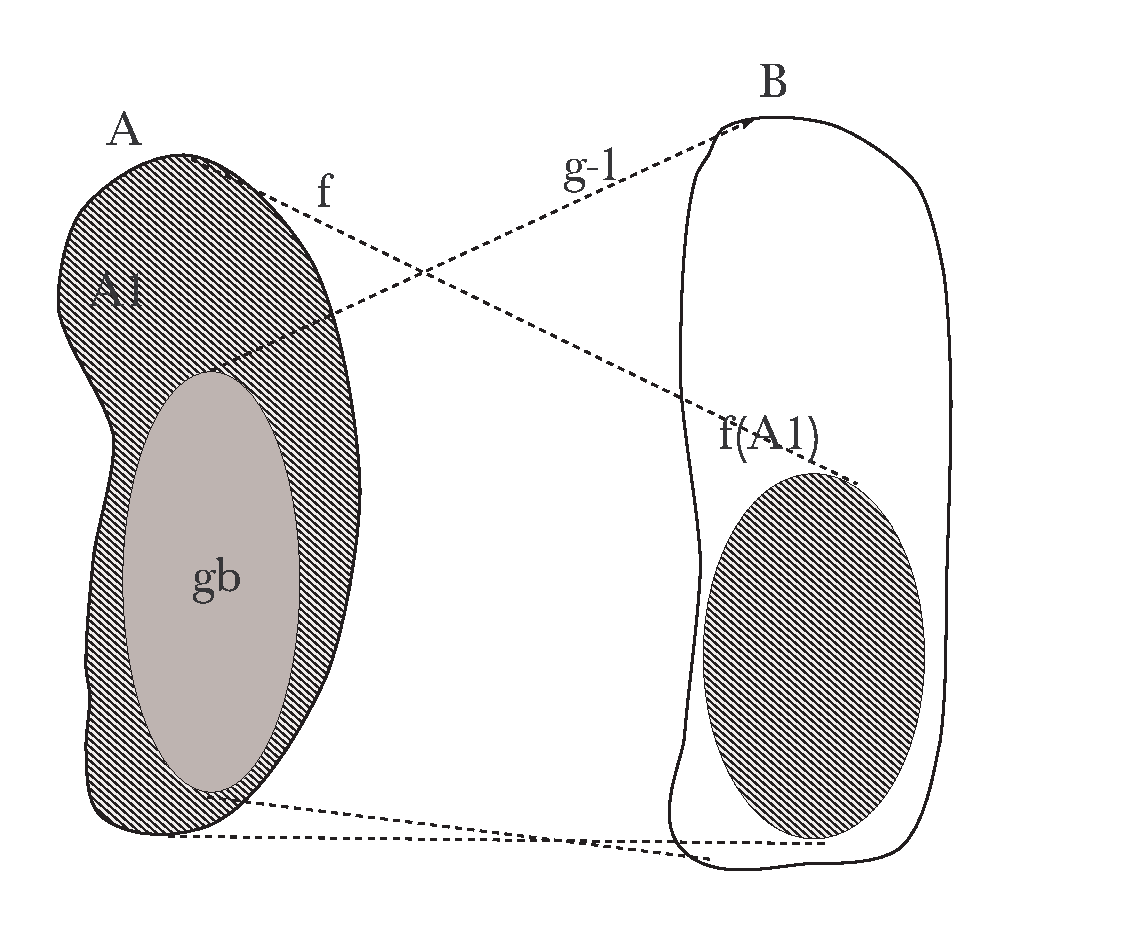
\includegraphics[height=10cm, width=10cm]{supfyg.eps}

\end{center}

 \caption{Las funciones $f$ y $g^{-1}$}\label{figura3}
\end{figure}

Una primera aproximaci\'on ser\'{\i}a intentar la construcci\'on
con $\tilde{A}=g(B)^c$. Seguramente as\'{\i} la funci\'on
$\tilde{f}$, ver ~\eqref{ftilde}, est\'a bien definida. La
funci\'on $\tilde{f}$ ser\'a suryectiva, pues $g^{-1}$ es
suryectiva de $g(B)$ en $B$. No obstante, con esa elecci\'on de
$\tilde{A}$, la funci\'on $\tilde{f}$ no es inyectiva, pues cada
elemento de $B_1$ es im\'agen, por esta $\tilde{f}$, de dos
elementos, uno en $A_1$ y otro en $g(B)$. De modo que esta
elecci\'on de $\tilde{A}$ todav\'{\i}a no nos sirve. Lo que vamos
a hacer ahora es agregarle a $\tilde{A}$ el conjunto de todos los
elementos de $g(B)$ tales que $g^{-1}$ los ``lleva'' a $B_1$. Este
conjunto es $A_2:=g(B_1)$. Definamos adem\'as $B_2:=f(A_2)$. Ahora
$\tilde{f}$ llevar\'a $A_1\cup A_2$ en $B_1\cup B_2$. Nos
preguntamos, ahora, si la elecci\'on $\tilde{A}:=A_1\cup A_2$ nos
servir\'a. Lamentablemente, la respuesta es
no\footnote{Podr\'{\i}a ser que si, si la funci\'on $f$ hubiera
sido biyectiva desde un principio, cosa que descartamos}. Al haber
``agrandado'' $\tilde{A}$ tambi\'en se nos agrand\'o el conjunto
de puntos en $B$ que son imagen de dos puntos, antes era el $B_1$,
ahora ``apareci\'o'' el $B_2$. De modo que continuamos el proceso,
es decir, definimos $A_3:=g(B_2)$, $B_3:=f(A_3)$ y as\'{\i}
sucesivamente, ver Figura \vref{figura4} . Nunca llegaremos, en
una cantidad finita de pasos, al conjunto $\tilde{A}$ con la
propiedad deseada, puesto que al cabo de $n$ pasos se nos genera
el conjunto $B_n$ donde las imagenes continuan superponiendos\'e.
?`Qu\'e haremos entonces?. Lo que se har\'a es seguir este proceso
indefinidamente, generando una sucesi\'on de conjuntos $A_n$ y
$B_n$, y luego definir:

\begin{equation}\label{defatilde}
\tilde{A}:=\bigcup_{n=1}^{\infty}A_n.
\end{equation}



\begin{figure}[h]

 \begin{center}

\psfrag{A}{$A$}

 \psfrag{B}{$B$}

 \psfrag{A1}{$A_1=A-g(B)$}
 \psfrag{A2}{$A_2=g(B_1)$}
 \psfrag{A3}{$ A_3=g(B_2)$}
\psfrag{B1}{$B_1=f(A_1)$}
 \psfrag{B2}{$B_2=f(A_2)$}
 \psfrag{B3}{$B_3=f(A_3)$}

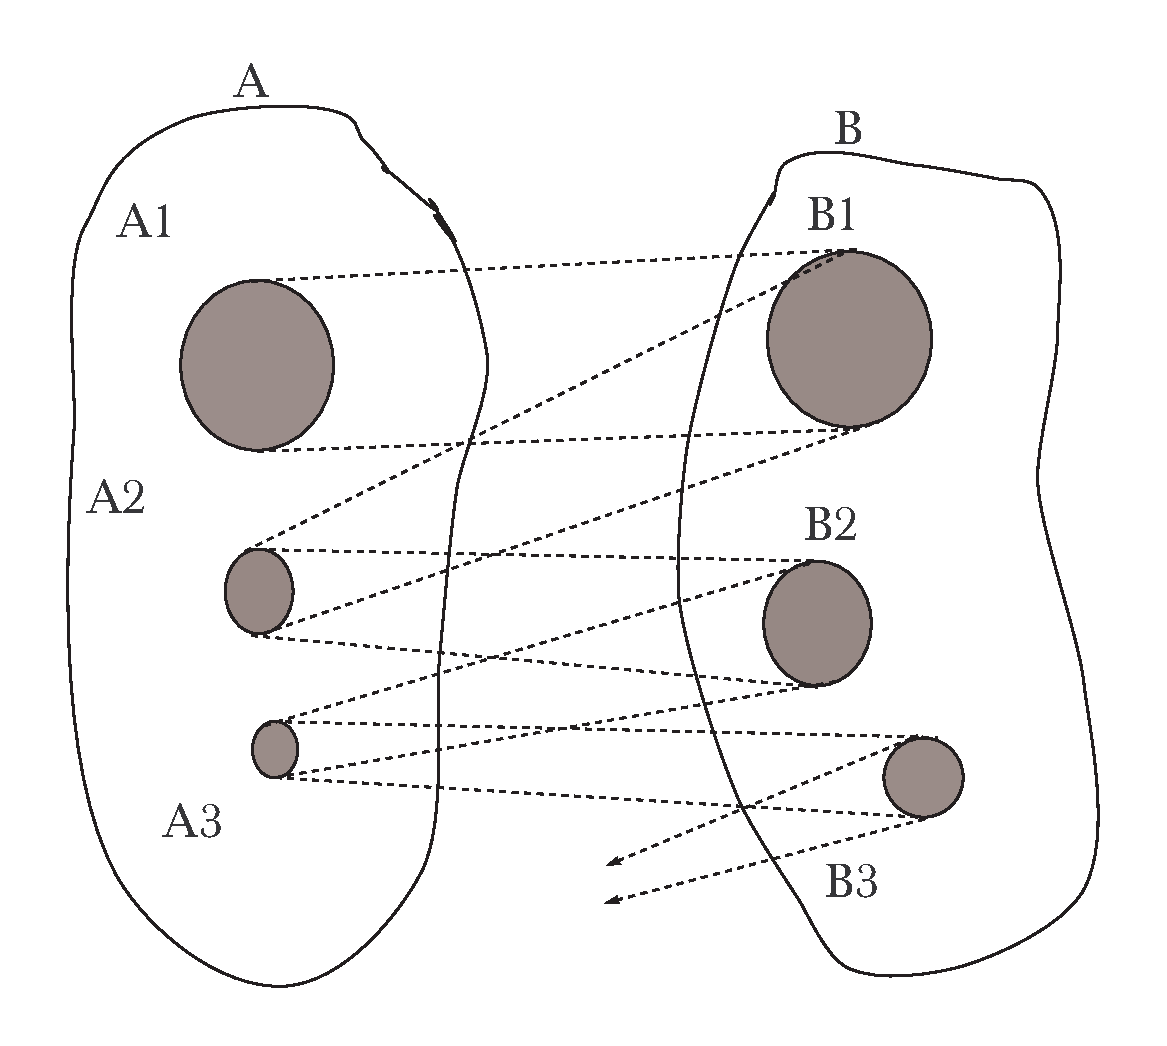
\includegraphics[height=10cm, width=10cm]{schber4.eps}

\end{center}

 \caption{Demostraci\'on del teorema de Schr\"oder-Berstein}\label{figura4}
\end{figure}

Intuitivamente, este conjunto deber\'{\i}a  funcionar, es decir no
hay m\'as superposici\'on de $f$ con $g^{-1}$. Esto es pues si
$a\in\tilde{A}$ entonces $a\in A_n$, para alg\'un $n$, y $f(a)\in
B_n$; eventualmente $f(a)$ podr\'{\i}a ser igual a alg\'un
$g^{-1}(a')$, pero $a'$ tendr\'{\i}a que estar en $A_{n+1}$ y por
consiguiente est\'a en $\tilde{A}$. Y as\'{\i}
$\tilde{f}(a')=f(a')$, y no $\tilde{f}(a')=g^{-1}(a')$, evitando
la superposici\'on de imagenes.

\vspace{10pt}
\begin{demo}\emph{Teorema \ref{scho-ber}} Estamos en condiciones de hacer la demostraci\'on propiamente
dicha del teorema. Hasta ahora solo tratamos de explicar la
demostraci\'on. Definimos inductivamente conjuntos $A_n$ y $B_n$
de la siguiente manera:

\[\left\{%
\begin{array}{ll}
    A_1=g(B)^c, & B_1=f(A_1) \\
    A_{n+1}=g(B_n), & B_{n+1}=f(A_{n+1}) \\
\end{array}%
\right..\]

Definamos $\tilde{A}$  como en ~\eqref{defatilde} y $\tilde{f}$
como en ~\eqref{ftilde}. Veamos que $\tilde{f}:A\longrightarrow B$
es biyectiva, empezando por la inyectividad.

Sean $a,a'\in A$ dos puntos cualesquiera tales que
$\tilde{f}(a)=\tilde{f}(a')$. Si $a$ y $a'$ est\'an
simultaneamente en $\tilde{A}$, o en $\tilde{A}^c$, tenemos que
$a=a'$ como consecuencia de que $f$, o $g^{-1}$, es inyectiva.
Consideremos, entonces, el caso $a\in\tilde{A}$ y $a'\notin
\tilde{A}$. Debemos llegar a una contradicci\'on pues estamos
suponiendo indirectamente que $a\neq a'$, por estar en conjuntos
disjuntos, y $\tilde{f}(a)=\tilde{f}(a')$. Tenemos que, para
alg\'un $n\in\nn$, $a\in A_n$; adem\'as, por la definici\'on de
$\tilde{f}$, tenemos que $f(a)=g^{-1}(a')$. Por consiguiente
$g(f(a))=a'$. Como $a\in A_n$, $f(a)\in B_n$ y $a'=g(f(a))\in
A_{n+1}$. Esto contradice que $a'\notin\tilde{A}$.

Veamos ahora la suryectividad. Sea $b\in B$ cualquier punto. Si
$b\in B_n$, para alg\'un $n$, como $B_n=f(A_n)$, ciertamente
existe un elemento $a\in A_n$ tal que $f(a)=b$. Ahora, por la
definici\'on de $\tilde{f}$, $\tilde{f}(a)=f(a)=b$. Supongamos,
pues, que $b$ no est\'a en ning\'un $B_n$. Como una afirmaci\'on
intermedia, probaremos que $g(b)$ no est\'a en ning\'un $A_n$.
Supongamos, por el contrario, que existe un $n$ tal que $g(b)\in
A_n$. Tiene que ser $n>1$, pues $A_1=g(B)^c$ y $g(b)\in g(B)$.
As\'{\i}, por su definici\'on  y como $n>1$, el conjunto $A_n$ es
igual a $g(B_{n-1})$. De modo que $g(b)\in g(B_{n-1})$. Esto
implica que existe un $b'\in B_{n-1}$ tal que $g(b)=g(b')$. Pero,
como $g$ es inyectiva $b=b'$ y, por ende, $b\in B_{n-1}$.
Contradiciendo esto que $b$ no estaba en ning\'un $B_n$. Probamos,
as\'{\i}, que $g(b)$ no est\'a en ning\'un $A_n$. Por lo tanto
$\tilde{f}(g(b))=g^{-1}(g(b))=b$. Vale decir $b=\tilde{f}(a)$ con
$a=g(b)$. Que era lo que quer\'{\i}amos probar.
\end{demo}

\section{Aplicaciones del Teorema de Schr\"oder-Berstein}

El teorema de Schr\"oder-Berstein es una herramienta potente para
probar coordinabilidad de conjuntos. En particular lo usaremos en
las cuestiones que a continuaci\'on exponemos. Hab\'{\i}amos visto
que $\rr\nsim\nn$. ?` Qu\'e ocurre con $\rr^2$, $\rr^3$,...?
?`Ser\'an estos conjuntos m\'as ``numerosos'' que $\rr$? Esto es:
?`Ser\'an no coordinables con $\rr$?. La respuesta a estas
preguntas es negativa, es decir $\rr^n\thicksim\rr$. Para ver esto
basta demostrar que $(0,1)^2\thicksim (0,1)$. El caso general es
consecuencia del caso $n=2$, usando inducci\'on, el Ejemplo
\vref{rcoord(0,1)} y el Ejercicio \vref{1.2}.

\begin{teorema} $(0,1)^2\thicksim (0,1)$.
\end{teorema}
\begin{demo} Observar que $(0,1)\precsim (0,1)^2$; podemos, para
demostrarlo, considerar la funci\'on inyectiva $f(x)=(x,1/2)$.

Veamos, ahora, que $(0,1)^2\precsim (0,1)$. Debemos construir una
funci\'on inyectiva $f:(0,1)^2\longrightarrow (0,1)$. Sea
$(x,y)\in (0,1)^2$. Consideremos las expresiones decimales
$x=0.x_1x_2...$ e $y=0.y_1y_2...$, donde $x_i$ e $y_i$ son enteros
entre 0 y 9, y no son todos 9 a partir de un momento en adelante.
Entonces escribimos:
\[f(x,y):=0.x_1y_1x_2y_2....\]
Es decir, $f$ intercala las expresiones decimales de $x$ e $y$.
Esta funci\'on es inyectiva, puesto que dos expresiones decimales
iguales tienen todos sus d\'{\i}gitos correspondientes iguales.
Esto concluye la demostraci\'on.
\end{demo}

Es bueno notar que la funci\'on $f$, definida en la demostraci\'on
anterior, no es suryectiva. Un n\'umero que no es imagen de
ning\'un par es $0.909090...$. ?`Por qu\'e ser\'a esto?

Por el Teorema \vref{teorcantor} tenemos que
$\nn\prec\mathcal{P}(\nn)$. Desmostramos, adem\'as, que $\nn\prec
\rr$. Nos preguntamos, ahora, que relaci\'on unir\'a
$\mathcal{P}(\nn)$ con $\rr$. Con el siguiente teorema probaremos
que aquellos conjuntos son coordinables.

\begin{teorema} $\mathcal{P}(\nn)\thicksim\rr$.
\end{teorema}
\begin{demo} Probaremos que $\mathcal{P}(\nn)\precsim\rr$ y despu\'es que
$\mathcal{P}(\nn)\succsim\rr$.

 Como $\mathcal{P}(\nn)\thicksim\mathbf{2}^{\nn}$ ( Ejercicio \vref{6}), y por el
 Ejercicio \vref{1.2} inciso 4, probaremos que $\mathcal{P}(\nn)\precsim\rr$ si podemos
 probar que $\mathbf{2}^{\nn}\precsim \rr$. Para este fin,
 consideremos la siguiente funci\'on:
 \[
    \begin{split}
          T:\mathbf{2}^{\nn}&\longrightarrow \rr\\
           f&\longmapsto 0.f(1)f(2)f(3)...\\
    \end{split}
 .\]
Esto es la funci\'on $f$ se aplica en un n\'umero cuya expansi\'on
decimal tiene solo ceros y unos. Esta funci\'on es inyectiva, pues
si
\[0.f(1)f(2)f(3)...=0.g(1)g(2)g(3)...\]
Entonces, por la unicidad de la expansi\'on
decimal\footnote{Recordemos que puede haber expresiones decimales
distintas que representan el mismo n\'umero, estas son las
expresiones que tienen todos nueves a partir de un momento en
adelante, como por ejemplo 1=0.999....No obstante este problema no
se nos presenta aqu\'{\i} pues la expresiones decimales que
consideramos tienen solo 0 y 1}, tenemos que $f(1)=g (1)$,
$f(2)=g(2)$,.... Por consiguiente las funciones son iguales. Lo
que prueba la inyectividad. De este modo demostramos que
$\mathbf{2}^{\nn}\precsim \rr$ y esto, por lo que explicamos
anteriormente, implica que $\mathcal{P}(\nn)\precsim \rr$

Ahora debemos ver que $\mathcal{P}(\nn)\succsim\rr$. Utilizando
los  incisos 1. y 4. del Ejercicios \vref{1.2}, vemos que es
suficiente probar que $\rr\precsim \mathcal{P}(\mathbb{Q})$. Para
hacer esto definimos la siguiente aplicaci\'on:
\[
   \begin{split}
        T:\rr &\longrightarrow \mathcal{P}(\mathbb{Q})\\
        r &\longmapsto \{q\in\mathbb{Q}:q<r\}
   \end{split}
.\]

Veamos que  la aplicaci\'on es inyectiva. Sean $r_1,r_2\in\rr$
n\'umeros reales distintos, supongamos $r_1<r_2$. Por la densidad
de $\mathbb{Q}$, existe un $q_0\in\mathbb{Q}$ tal que
$q_0\in(r_1,r_2)$. As\'{\i} $q_0\in\{q\in\mathbb{Q}:q<r_2\}$ y
$q_0\notin\{q\in\mathbb{Q}:q<r_1\}$. De modo que
\[\{q\in\mathbb{Q}:q<r_1\}\neq\{q\in\mathbb{Q}:q<r_2\}.\]
Es decir $T$ es inyectiva.
\end{demo}
Para finalizar demostraremos que
$\nn^{\nn}\thicksim\mathbf{2}^{\nn}$. Mas que el resultado en
s\'{\i}, vamos a resaltar su demostraci\'on, pues contiene una
idea interesante.

\begin{proposicion} $\nn^{\nn}\thicksim\mathbf{2}^{\nn}$.
\end{proposicion}

\begin{demo} Dado un conjunto $X$ cualquiera, podemos interpretar una
funci\'on $f\in X^{\nn}$ como una sucesi\'on de elementos de $X$,
a la que podemos disponer de la siguiente manera:
\begin{equation}\label{mensajes}
     f=(f(1),f(2),f(3),...).
\end{equation}
Si $X=\nn$ entonces la sucesi\'on ser\'a de n\'umeros naturales y
si $X=\mathbf{2}$ entonces la sucesi\'on ser\'a de ceros y unos.

Interpretemos el segundo miembro de ~\eqref{mensajes}  como una
palabra infinita. Si $X=\nn$, esta palabras se compone de
``letras'' que pueden ser cualquier n\'umero natural. Si
$X=\mathbf{2}$, esta ``palabra'' se escribe con solo dos
``letras'' el 0 y el 1. La pregunta es: ?`C\'omo podemos
``traducir'' una palabra escrita con un alfabeto de infitas
letras, a uno con solo dos?. La soluci\'on a esto es ingeniosa.
Sea $f\in\nn^{\nn}$, usaremos el signo 1 para denotar las comas en
la sucesi\'on $f$ y pondr\'emos tantos ceros como indiquen las
cantidades $f(j)$.


\[
  \begin{split}
         T\quad:\quad\nn^{\nn}\quad\quad &\longrightarrow\quad\quad\mathbf{2}^{\nn}\\
         f=(f(1),f(2),f(3),...)&\longmapsto
          (\underbrace{0,...,0}_{f(1)\,\,\text{ceros}},1,
          \underbrace{0,...,0}_{f(2)\,\,\text{ceros}},1,....)\\
 \end{split}
\]
Veamos que esta funci\'on es inyectiva. Sean $f,g\in\nn^{\nn}$,
con  $f\neq g$. Sea
\[j=\min\{i:f(i)\neq g(i)\}.\]
Tenemos que $f(i)=g(i)$ para $i<j$. Escribamos las dos sucesiones

\[   (\underbrace{0,...,0}_{f(1)\,\,\text{ceros}},1,
         ...,1,\underbrace{0,...,0}_{f(j-1)
          \,\,\text{ceros}},1, \underbrace{0,...,0}_{f(j)\,\,\text{ceros}},1,....)
\]
y
\[   (\underbrace{0,...,0}_{g(1)\,\,\text{ceros}},1,
         ...,1,\underbrace{0,...,0}_{g(j-1)
          \,\,\text{ceros}},1, \underbrace{0,...,0}_{g(j)\,\,\text{ceros}},1,....)
\]
Notar que los primeros $j-1$ grupos de ceros son iguales, pues
$f(i)=g(i)$ para $i<j$, por consiguiente los primeros $j-1$ unos
estan en la misma posici\'on en las dos sucesiones. Pero $f(j)\neq
g(j)$ y, por consiguiente, el grupo $j$-\'esimo de ceros debe
diferir en las dos sucesiones. Esto fuerza que si, por ejemplo,
$f(j)<g(j)$, entonces la sucesi\'on $f$ tendr\'a un uno donde la
$g$ tiene un cero.

As\'{\i} $T(f)\neq T(g)$ y la funci\'on es inyectiva. Esto prueba
que $\nn^{\nn}\precsim \mathbf{2}^{\nn}$. La otra desigualdad es
m\'as f\'acil de obtener pues
\[
  \begin{split}
      \mathbf{2}&\precsim \nn\quad\,\,\, \text{pues unos es finito y el
      otro no}\\
      \mathbf{2}^{\nn}&\precsim\nn^{\nn}\quad \text{por el
      Ejercicio \ref{potdelapot} }
  \end{split}
\]
\end{demo}

Existe una demostraci\'on m\'as sucinta de que
$\nn^{\nn}\precsim\mathbf{2}^{\nn}$. No la preferimos debido a que
no muestra una biyecci\'on, es una demostraci\'on indirecta. Ahora
la exponemos.
\[
  \begin{split}
       \nn &\precsim \mathbf{2}^{\nn}\quad\quad\,\text{Teorema de
       Cantor}\\
       \nn^{\nn} &\precsim (\mathbf{2}^{\nn})^{\nn}\quad\text{Ejercicio
       \ref{potdelapot}}\\
        \nn^{\nn} &\precsim \mathbf{2}^{\nn\times\nn}\quad\,\text{Ejercicio
       \ref{potdelapot}}\\
        \nn^{\nn} &\precsim \mathbf{2}^{\nn}\quad\quad\,\text{Proposici\'on  \ref{NxNesnum}}\\
        \nn^{\nn} &\precsim \mathbf{2}^{\nn}\quad\quad\,\text{Ejercicio
       \ref{1.2} inciso 3}.
  \end{split}
\]


\section{Ejercicios}


\begin{ejercicio}\label{propuniarb} Sea $f:A\longrightarrow B$ una funci\'on cualquiera.
Supongamos que $\{A_i\}_{i\in I}$ y $\{B_i\}_{i\in I}$ son
familias subindicadas de conjuntos, donde los $A_i$ y $B_i$ son
subconjuntos de $A$ y $B$ respectivamente. Demostrar las
siguientes propiedades:
\end{ejercicio}
\begin{itemize}
\item[1.] $\biggl(\bigcup_{i\in I}A_i\biggr)^c=\bigcap_{i\in
I}A_i^c$.
\item[2.]$\biggl(\bigcap_{i\in I}A_i\biggr)^c=\bigcup_{i\in
I}A_i^c$.
\item[3.] $f\biggl(\bigcup_{i\in I}A_i\biggr)=\bigcup_{i\in
I}f(A_i)$.
\item[4.]?`Qu\'e ocurre con $f\biggl(\bigcap_{i\in I}A_i\biggr)$?
\item[5.] $f^{-1}\biggl(\bigcup_{i\in I}B_i\biggr)=\bigcup_{i\in
I}f^{-1}(B_i)$.
\item[6.]$f^{-1}\biggl(\bigcap_{i\in I}B_i\biggr)=\bigcap_{i\in
I}f^{-1}(B_i)$.
\end{itemize}

\begin{ejercicio}\label{3} Demostrar las propiedades de la
Proposici\'on \vref{propfunc}
\end{ejercicio}
\begin{ejercicio}\label{1} Probar que $\thicksim$ es una
relaci\'on de equivalencia.
\end{ejercicio}
\begin{ejercicio}\label{1.2} Supongamos que $A\thicksim B$ y
$C\thicksim D$.
\begin{itemize}
\item[1.] Demostrar que $\mathcal{P}(A)\thicksim \mathcal{P}(B)$.
\item[2.] Demostrar que $A\times C\thicksim B\times D$.
\item[3.] Demostrar que $A^C\thicksim B^D$.
\item[4.] Si $A\precsim C$ entonces $B\precsim D$.
\end{itemize}
\end{ejercicio}
\begin{ejercicio}\label{potdelapot} Sean $A$, $B$ y $C$ conjuntos
no vacios. Demostrar que
\begin{itemize}
\item[1.] $\bigl(A^{B}\bigr)^C\thicksim A^{B\times C}$.
\item[2.] Si $A\precsim B$ entonces $A^C\precsim B^C$.
\end{itemize}
\end{ejercicio}

\begin{ejercicio}\label{1.5} Demostrar que un subconjunto de un conjunto
finito es finito.
\end{ejercicio}
\begin{ejercicio}\label{2} Demostrar que la funci\'on
$f:\nn\times\nn\longrightarrow\nn$ definida por:
\[f(j,k):=\frac{(j+k-1)(j+k)}{2}-j+1,\]
es una biyecci\'on.
\end{ejercicio}
\begin{ejercicio}\label{5} Demostrar, exhibiendo una biyecci\'on, que $(0,1)\thicksim [0,1]$
\end{ejercicio}
\begin{ejercicio}\label{6} Demostrar que el conjunto
$\mathcal{P}(\nn)$ es coordinable con el conjunto
$\mathbf{2}^{\nn}$, donde $\mathbf{n}=\{0,1,...,n-1\}$. Recordar
que, si $A$ y $B$ son conjuntos, $B^A:=\{f:f:A\longrightarrow
B\}$. De este modo $\mathbf{2}^{\nn}$ es el conjunto de funciones
$f:\nn\longrightarrow \{0,1\}$.
\end{ejercicio}

\begin{ejercicio}\label{8} Demostrar que, para cualquier conjunto
$A$, $\mathcal{P}(A)\thicksim\mathbf{2}^A$.
\end{ejercicio}
\begin{ejercicio}\label{infcoordconsub} Demostrar que son
equivalentes:
\begin{itemize}
     \item[1.] $A$ es infinito.
     \item[2.] $A$ es coordinable con un subconjunto propio, es
     decir: Existe $B\subset A$, con $B\neq A$, tal que
     $A\thicksim B$.
\end{itemize}
\end{ejercicio}
\begin{ejercicio} Demostrar que el conjunto formado por todos los
sub-\newline conjuntos de $\nn$ que son finitos, es numerable.
?`Qu\'e ocurrira con el conjunto de todos los subconjuntos
infinitos?
\end{ejercicio}
\begin{ejercicio} Sea $\{A_i\}_{i\in I}$ una familia de intervalos
de $\rr$. Suponer que los conjuntos en la familia son mutuamente
disjuntos, es decir: $A_i\cap A_j=\emptyset$ si $i\neq j$.
Demostrar que el conjunto $\{A_i:i\in I\}$ es a lo sumo numerable.
\end{ejercicio}
\begin{ejercicio} Recordemos que una funci\'on
$f:\rr\longrightarrow\rr$ se dice nodecre-\newline ciente, si para
todos $x,y\in\rr$, tales que $x<y$, se tiene que $f(x)\leq f(y)$.
Dada una funci\'on nodecreciente, demostrar que el conjunto de
todos los puntos de discontinuidad es a lo sumo numerable.
\textit{Ayuda}: Demostrar en primera instancia que los
l\'{\i}mites laterales:
\[
    \lim\limits_{x\rightarrow a^+}f(x)\quad\text{y}\quad \lim\limits_{x\rightarrow
    a^-}f(x)
\]
existen para todo $a\in\rr$. Luego aplicar el ejercicio anterior.
\end{ejercicio}
\begin{ejercicio} Demostrar que $\rr^{\nn}\thicksim\rr$.
\end{ejercicio}
\begin{ejercicio} Como aprendimos $\nn\thicksim\mathbb{Q}$, esto
significa que existe una aplicaci\'on biyectiva
$f:\nn\longrightarrow\mathbb{Q}$, que nos permite enumerar
$\mathbb{Q}$ como una suceci\'on $r_j:=f(j)$. Definimos la
aplicaci\'on:
\[\begin{split}
              T:C(\rr)&\longrightarrow \rr^{\nn}\\
              f        &\longmapsto T_f\\
\end{split}\]
donde
\[
  T_f(j):=f(r_j).
\]
\begin{itemize}
   \item [1.] Demostrar que $T$ es inyectiva. Por consiguiente
   $C(\rr)\precsim\rr^{\nn}$.
   \item[2.] Usando el inciso anterior, demostrar que
    $C(\rr)\thicksim\rr$, donde $C(\rr)$ es el conjunto
    de las funciones continuas de $\rr$ en si mismo.
\end{itemize}
\end{ejercicio}
